\documentclass[10pt]{article}
% Math Packages
\usepackage{amsmath, mathtools}
\usepackage{amssymb}
\usepackage{amsthm}
\usepackage{amsfonts}
\usepackage{bbm}
\usepackage{breqn}
\usepackage[margin=1in]{geometry}
\usepackage{graphicx}
\usepackage{tikz}
\usetikzlibrary{arrows.meta}
\usetikzlibrary{calc}
\usepackage{forest}
\usepackage{tikz-qtree}
\graphicspath{ {./images/} }
\usepackage{hyperref}
\usepackage[capitalize]{cleveref}
\usepackage[shortlabels]{enumitem}
\usetikzlibrary{arrows,matrix,positioning}
\usepackage{multicol}

% for the pipe symbol
\usepackage[T1]{fontenc}

% Citing theorems by name. (source: https://tex.stackexchange.com/questions/109843/cleveref-and-named-theorems)
\makeatletter
\newcommand{\ncref}[1]{\cref{#1}\mynameref{#1}{\csname r@#1\endcsname}}

\def\mynameref#1#2{%
  \begingroup
  \edef\@mytxt{#2}%
  \edef\@mytst{\expandafter\@thirdoffive\@mytxt}%
  \ifx\@mytst\empty\else
  \space(\nameref{#1})\fi
  \endgroup
}
\makeatother

% Colorful Notes
\usepackage{color} \definecolor{Red}{rgb}{1,0,0} \definecolor{Blue}{rgb}{0,0,1}
\definecolor{Purple}{rgb}{.5,0,.5} \def\red{\color{Red}} \def\blue{\color{Blue}}
\def\gray{\color{gray}} \def\purple{\color{Purple}}
\newcommand{\rnote}[1]{{\red [#1]}} % \rnote{foo} gives '[foo]' in red
\newcommand{\pnote}[1]{{\purple [#1]}} % \pnote{foo} gives '[foo]' in purple
\newcommand{\bnote}[1]{{\blue #1}} % \bnote{foo} gives 'foo' in blue
\newcommand{\gnote}[1]{{\gray #1}} % \gnote{foo} gives 'foo' in gray
\newcommand{\Max}[1]{{\purple [#1]}} % \bnote{foo} then 'foo' is blue


% Claim numbering (the counter restarts after each proof environment)
\newcounter{claimcount}
\setcounter{claimcount}{0}
\newenvironment{claim}{\refstepcounter{claimcount}\par\addvspace{\medskipamount}\noindent\textbf{Claim \arabic{claimcount}:}}{}
\usepackage{etoolbox}
\AtBeginEnvironment{proof}{\setcounter{claimcount}{0}}
\newenvironment{claimproof}{\par\addvspace{\medskipamount}\noindent\textit{Proof of Claim  \arabic{claimcount}.}}{\hfill\ensuremath{\qedsymbol} \tiny{Claim}

  \medskip}
% Add claim support to cleverref
\crefname{claimcount}{Claim}{Claims}


% Math Environments
\newtheorem{theorem}{Theorem}
\newtheorem{assumption}[theorem]{Assumption}
\newtheorem{lemma}[theorem]{Lemma}
\newtheorem{proposition}[theorem]{Proposition}
\newtheorem{corollary}[theorem]{Corollary}
\newtheorem{question}[theorem]{Question}
\theoremstyle{definition}
\newtheorem{definition}[theorem]{Definition}
\newtheorem{remark}[theorem]{Remark}
\newtheorem{example}[theorem]{Example}
\newtheorem{notation}[theorem]{Notation}
\newtheorem{problem}[theorem]{Problem}

% Matrices and Column Vectors. 
\usepackage{stackengine}
\setstackgap{L}{1.0\normalbaselineskip}
\usepackage{tabstackengine}
\setstackEOL{;}% row separator
\setstackTAB{,}% column separator
\setstacktabbedgap{1ex}% inter-column gap
\setstackgap{L}{1.5\normalbaselineskip}% inter-row baselineskip
\let\nmatrix\bracketMatrixstack  %Usage: \nmatrix{1,2,3\4,5,6}
\newcommand\cv[1]{\setstackEOL{,}\bracketMatrixstack{#1}} %usage: \cv{1,2,3}

% Custom Math Coqmmands
\newcommand{\vt}{\vskip 5mm} % vertical space
\newcommand{\fl}{\noindent\textbf} % first line
\newcommand{\Fl}{\vt\noindent\textbf} % first line with space above
\newcommand{\norm}[1]{\left\lVert#1\right\rVert} % norm
\newcommand{\pnorm}[1]{\left\lVert#1\right\rVert_p} % p-norm
\newcommand{\qnorm}[1]{\left\lVert#1\right\rVert_q} % q-norm
\newcommand{\1}[1]{\textbf{1}_{\left[#1\right]}} % indicator function 
\def\limn{\lim_{n\to\infty}} % shortcut for lim as n-> infinity
\def\sumn{\sum_{n=1}^{\infty}} % shortcut for sum from n=1 to infinity
\def\sumkn{\sum_{k=1}^{n}} % shortcut for sum from k=1 to n
\def\sumin{\sum_{i=1}^{n}} % shortcut for sum from i=1 to n
\def\SAs{\sigma\text{-algebras}} % shortcut for $\sigma$-algebras
\def\SA{\sigma\text{-algebra}} % shortcut for $\sigma$-algebra
\def\Ft{\mathcal{F}_t} % time-indexed sigma-algebra (t)
\def\Fs{\mathcal{F}_s} % time-indexed sigma-algebra (s)
\def\F{\mathcal{F}} % sigma-algebra
\def\G{\mathcal{G}} % sigma-algebra
\def\R{\mathbb{R}} % Real numbers
\def\N{\mathbb{N}} % Natural numbers
\def\Z{\mathbb{Z}} % Integers
\def\E{\mathbb{E}} % Expectation
\def\P{\mathbb{P}} % Probability
\def\Q{\mathbb{Q}} % Q probability
\def\dist{\text{dist}} %Text 'dist' for things like 'dist(x,y)'
\newcommand{\indep}{\perp \!\!\! \perp}  %independence symbol
\def\Var{\mathrm{Var}} % Variance
\def\tr{\mathrm{tr}} % trace

% Brackets and Parentheses
\def\[{\left [}
    \def\]{\right ]}
% \def\({\left (}
%   \def\){\right )}



\usepackage{color}
\definecolor{Red}{rgb}{1,0,0}
\definecolor{Blue}{rgb}{0,0,1}
\definecolor{Purple}{rgb}{.5,0,.5}
\def\red{\color{Red}}
\def\blue{\color{Blue}}
\def\gray{\color{gray}}
\def\purple{\color{Purple}}
\definecolor{RoyalBlue}{cmyk}{1, 0.50, 0, 0}
\newcommand{\dempfcolor}[1]{{\color{RoyalBlue}#1}} 
\newcommand{\demph}[1]{\dempfcolor{{\sl #1}}}

% comment exactly one of the following line to show / hide the solutions
% \newcommand{\solution}[1]{{\purple #1}} % uncomment to show the solutions
\newcommand{\solution}[1]{} % uncomment to hide the solutions



\title{Lecture Notes for Math 372: \\Elementary Probability and Statistics}
\date{Last updated: \today}
% \author{mh}

\begin{document}
\begin{center}
  \section*{Math 372: Homework 02}
  \textit{Due Wednesday, Jan 28}
\end{center}
\begin{problem}[Sets]
  A consulting firm has bids on 3 projects. Let
  \begin{equation*}
    A_{i} = \left[ \text{awarded project } i \right] 
  \end{equation*}
  for $i\in \left\{1,2,3\right\}$. Suppose that
  \begin{gather*}
    \P\left[A_{1} \right]= .22\\
    \P\left[A_{2} \right]= .25\\
    \P\left[A_{3} \right]= .28\\
    \P\left[A_{1}\cap A_{2} \right]= .11\\
    \P\left[A_{1}\cap A_{3} \right]= .05\\
    \P\left[A_{2}\cap A_{3} \right]= .07\\
    \P\left[A_{1}\cap A_{2}\cap A_{3} \right]= .01
  \end{gather*}

  \begin{enumerate}[(a)]
    \item In the following Venn diagram, the three overlapping circles represent events $A_{1},A_{2},$ and
    $A_{3}$, all contained within the sample space box $S$. Each enclosed region represents an event, all
    of which have some probability of occurring. I've already filled in the probability of one of the
    events (namely, the event $A_{1}\cap A_{2}\cap A_{3}$). Using the probabilities above, fill in the
    probabilities of other 7 regions:
    \begin{center}
      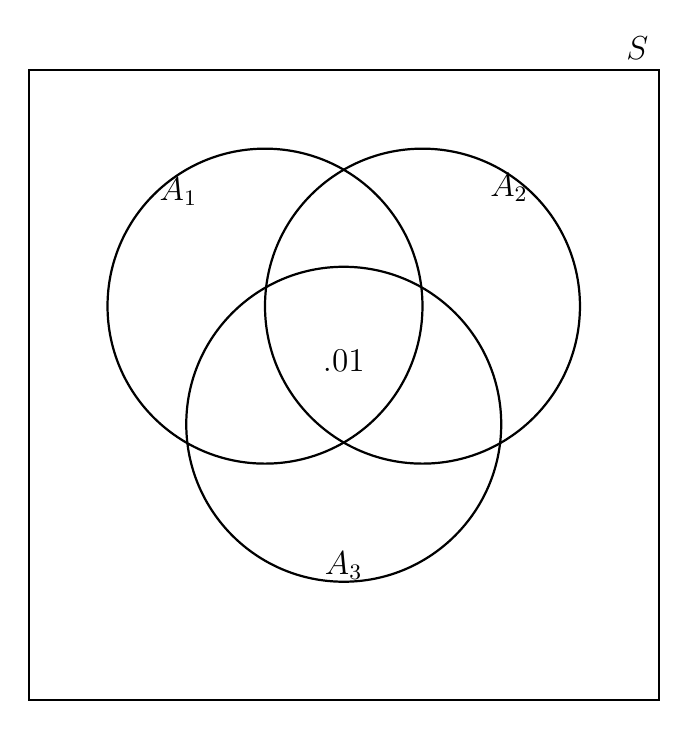
\begin{tikzpicture}
        % Draw the rectangular box
        \draw[thick] (-3, -5) rectangle (5, 3) node[above left] {\large $S$};
        % Define circles
        \draw[thick] (0,0) circle (2cm);
        \draw[thick] (2,0) circle (2cm);
        \draw[thick] (1,-1.5) circle (2cm);
        % Add labels for sets
        \node at (-1.1, 1.45) {\large $A_{1}$};
        \node at (3.1, 1.5) {\large $A_{2}$};
        \node at (1, -3.3) {\large $A_{3}$};
        \node at (1, -0.70) {\large $.01$};
      \end{tikzpicture}
    \end{center}

    \item Express in words each of the following events, and compute the probability of each event:
    \begin{enumerate}[(i.)]
      \item $A_{1}\cup A_{2} $
      \item $A_{1}^{c}\cap A_{2}^{c}$ \textit{[Hint: use De Morgan's laws.
        Note: the textbook uses the notation $A'_{i}$ in place of
        $A_{i}^{c}$.]}
      \item $A_{1}\cup A_{2}\cup A_{3}$
      \item $A_{1}^{c}\cap A_{2}^{c}\cap A_{3}^{c}$
      \item $A_{1}^{c}\cap A_{2}^{c}\cap A_{3} $
      \item $\left( A_{1}^{c}\cap A_{2}^{c} \right)\cup A_{3}$
    \end{enumerate}
  \end{enumerate}
\end{problem}

\begin{problem}[Sets]
  Suppose that $55\%$ of all people regularly consume coffee, $45\%$ regularly consume soda, and $70\%$
  regularly consume at least one of these two drinks. \textit{[Hint: draw a Venn diagram.]}
  \begin{enumerate}[(a.)]
    \item What is the probability that a randomly-selected person consumes both coffee and soda?
    \item What is the probability that a randomly-selected person doesn't regularly consume at least one
    of these drinks?
  \end{enumerate}
\end{problem}

\begin{problem}[The geometric distribution]
  \label{problem:geometric-experiment}
  Suppose we have an urn containing exactly $3$ balls: two white balls and one
  gold ball. Consider the experiment specified by the following algorithm:
\begin{verbatim}
      Algorithm:

      Step 1. Draw a ball at random from the urn.

      Step 2. If you drew the gold ball, stop. Otherwise, put the
              ball back into the urn and return to step 1.

      Output: the number of times X you drew a ball from the urn.
\end{verbatim}
  In other words, you repeatedly draw a ball from the urn at random until you
  get the gold ball, where, if you draw a white ball, you have to put it back
  and draw again. The output is the (random) quantity $X$, which is the number
  of times you drew a ball in this process.

  \begin{enumerate}[(a.)]
    \item Find a way to actually run this experiment, and repeat it 10 times.
    Record (i) how you did it, (ii) the ten outputs you got, and (iii) their
    average.
    
    \item What is the sample space $S$ of this experiment? What possible
    values can $X$ take?
    \item Compute following probabilities: $\P\left[X=1 \right]$,
    $\P\left[X=2 \right]$, $\P\left[X=3 \right]$, $\P\left[X=4 \right]$,
    $\P\left[X=5 \right]$,
    \item Give a formula for $\P\left[X=n \right]$, where $n$ is a positive
    integer.
    \item Write the event $\left[ X \leq 5\right]$ as a subset of the sample
    space $S$ . Compute
    $\P\left[X \leq 5\right]$.
    \item Write the event $\left[ X \text{ is even} \right]$ as a subset of the
    sample space. Use the \textit{geometric series formula}
    \begin{equation*}
      1+x+x^{2}+x^{3}+x^{4}+\ldots = \frac{1}{1-x} \quad (\text{valid whenever }|x|<1)
    \end{equation*}
    to compute $\P\left[X \text{ is odd} \right]$.
    
    \item Compute $\E\left[X \right]$, the expectation of $X$. Use the formula
    \begin{equation*}
      \E\left[X \right]= \sum_{n=1}^{\infty} n \P\left[X=n \right].
    \end{equation*}
    Compare with your answer to part (iii) of (a).
  \end{enumerate}
\end{problem}

\begin{problem}[Counting]
  How many 7-character license plates are possible if the first 3 are to be
  occupied by letters and the final 4 by numbers? % ans: 175,760,000
\end{problem}


\begin{problem}[Counting]
  How many ways can you get dealt 5 cards containing exactly 2 jacks?
  % \begin{equation*}
  %   \underbrace{{48\choose 3}}_{\text{3 out of 48 non-jacks}}\times \underbrace{{4\choose 2}}_{\text{2
  %   out of 4 jacks}} = 103,776
  % \end{equation*}
\end{problem}




\begin{problem}[Counting]
  How many ways are there of flipping 10 coins and getting $5$ heads? What is the probability of
  this occurring?
  % ${10\choose 5} = 252$.
\end{problem}


\begin{problem}[Disjoint events]
  Suppose I have an urn with $6$ balls, labeled $1,\ldots,6$. If I draw two balls, what is the probability
  that they are either (1) both even or (2) both odd?
  % \begin{equation*}
  %   \P\left[\text{both even or both odd} \right]\overset{*}{=}
  %   \P\left[\text{both even}| \right] + \P\left[ \text{both odd} \right]
  %   = \frac{3}{15} + \frac{3}{15}=\frac{2}{5}
  % \end{equation*}
  % Equality $*$ is justified because
  % $\left[ \text{both even} \right]\cap \left[ \text{both odd} \right] = \emptyset$.
\end{problem}



\begin{problem}[Counting]
  A dessert company has 31 distinct desserts on its menu: 5 types of pie, 9 types of cake, and 17 flavors of ice
  cream. \textit{(You don't need to simplify your answers for this problem)}
  \begin{enumerate}[(a)]
    \item After purchasing 4 different desserts, a customer decides he will eat them all in a row, and he
    cares about the order in which he eats them. How many different ways can he eat his 4 desserts?
    \item Suppose 7 different desserts are selected from the menu. How many ways are there to do
    this if (i) we care about the order in which the 7 deserts are selected, and (ii) if we don't care
    about the order? 
    \item If 9 desserts are randomly selected, how many ways are there to obtain 3 deserts of each type
    (pie, cake, and ice cream)?
    \item If 5 desserts are randomly selected, what's the probability that they are all of the same
    type  (i.e., all pie, all cake, or all ice cream)?
  \end{enumerate}
\end{problem}



\begin{problem}
  Consider randomly selecting a student at a large university. Let $A$ be the
  event that the selected student has a Visa card and $B$ be the event that
  the student has a MasterCard. Suppose that $\P\left[A \right]=.6$ and
  $\P\left[B \right]=.4$
  \begin{enumerate}[(a)]
    \item Could it be the case that $\P\left[A\cap B \right] = .5$? Why or why
    not?
    \item From now on, suppose that $\P\left[A\cap B \right]=.3$. What is the
    probability that the selected student has at least one of these two types
    of cards?
    \item What is the probability that the selected student has neither type
    of card?
    \item Describe, in terms of $A$ and $B$, the event that the student has a
    Visa card but not a MasterCard. Then calculate the probability of this
    event.
    \item Calculate the probability that the selected student has exactly one
    of the two types of cards.
  \end{enumerate}
\end{problem}

\end{document}